\documentclass[12pt]{article}

\usepackage{sbc-template}

\usepackage{listings} %code
\usepackage{syntax} %grammar
\usepackage{graphicx,url} %figures
\usepackage{lscape}

\usepackage[utf8]{inputenc}
\usepackage[T1]{fontenc}
% UTF-8 encoding is recommended by ShareLaTex

\usepackage{algorithm2e}

\sloppy

\title{Anotações sobre Deep Neuroevolution}

\author{Ricardo Henrique Remes de Lima \inst{1}}

\address{Departamento de Informática\\
	Universidade Federal do Paraná (UFPR)\\
  \email{ricardo.hrlima@gmail.com}
}

\begin{document} 

\maketitle

\section{Convolutional Neural Networks}

\section{Deep Neuroevolution}

\section{Approach}

This section will present the details about the proposed approach, describing the tools used, the design of the grammar, how the mapping process creates the CNNs and how the search engine works to improve the solutions.

\subsection{Tools}

Here we present the tools that were used in order to better understand the decisions made in further steps of the approach. The technologies used are listed below:

\begin{itemize}
	\item \textbf{Python v3.6}: The use of the Python\footnote{https://www.python.org} language is supported by the well known frameworks that are used in machine learning projects, as well as offering a simple syntax to improve productivity. 
	
	\item \textbf{Tensorflow}: The Tensorflow\footnote{https://www.tensorflow.org} framework is a powerful open-source library for high performance numerical computation. Its flexible architecture allows easy deployment of computation across a variety of platforms.
	
	\item \textbf{Keras}: A Python Deep Learning library. Keras \footnote{https://keras.io/} is a high-level neural networks API, written in Python and capable of running on top of Tensorflow, CNTK\footnote{https://github.com/Microsoft/cntk} or Theano\footnote{https://github.com/Theano/Theano}. Designed to enable fast experimentation.
\end{itemize}


\subsection{Grammar}


The GE Grammar has the task of defining a generic structure that allows the creation of different variations of a program according to the problem. The rules and productions are usually used to describe ``blocks'' of routines and parameters that the program has, and also how these blocks connect to each other.


To design the CNNs we selected some of the most common layers implemented in the Keras framework, as well as some of the available parameters that comes with them. The options are listed below:


\begin{itemize}
	\item Convolution Layer: Filters, Kernel size, Activation function
	
	\item Max/ Average Pooling: Pooling size, Padding
	
	\item Dense: Units, Activation function
	
	\item Dropout: Drop rate
	
	\item Filters: 32, 64
	
	\item Kernel size: (3, 3), (5, 5)
	
	\item Activation function: Relu, Tahnm, Linear
	
	\item Pooling size: (2, 2), (4, 4)
	
	\item Padding: Valid, Same
	
	\item Number of Units: 32, 64
	
	\item Drop rate: rand[0, 1]
\end{itemize}


A first version of a grammar using the CNN components can be seen in Figure \ref{fig:cnn-grammar}. The rules and productions were designed to ensure the creation of valid CNN models, as well as giving the opportunity to grow in size and complexity.


\begin{figure}[!htb]
	\begin{grammar}
		<cnn> ::= <conv> <c\_layer> <d\_layer> <dense>
		
		<c\_layer> ::= <c\_layer> <c\_layer> | <c\_node> | '\&'
		
		<d\_layer> ::= <d\_node> <d\_node> | <d\_node> | '\&'
		
		<c\_node> ::= <conv> | <maxpool> | <avgpool>
		
		<d\_node> ::= <dense> | <dropout>
		
		<conv> ::= `Conv2D' <filters> <k\_size> <activation>
		
		<dense> ::= `Dense' <units>
		
		<dropout> ::= `Dropout' <rate>
		
		<maxpool> ::= `MaxPooling2D' <p\_size> <padding>
		
		<avgpool> ::= `AveragePooling2D' <p\_size> <padding>
		
		<activation> ::= `relu' | `tanh' | `linear'
		
		<padding> ::= `valid' | `same'
		
		<filters> ::= `32' | `64'
		
		<k\_size> ::= `(3, 3)' | `(5, 5)'
		
		<p\_size> ::= `(2, 2)' | `(4, 4)'
		
		<units> ::= `32' | `64'
		
		<rate> ::= `[0.0, 1.0]'
		
	\end{grammar}
	\caption{Proposed grammar to generate CNNs.}
	\label{fig:cnn-grammar}
\end{figure}


\subsection{Mapping}


The mapping is responsible to translate the genotype of a solution into the correspondent phenotype through the grammar. Generating CNNs with this approach is very simple, because we just have to define which layers will be used, in which sequence and also define the values of the parameters of each of these layers.


The proposed grammar was designed to allow the creation of both a small CNN with just one \textit{convolution} layer and one \textit{dense} layer, as well as CNNs as big as we want, using many \textit{convolution}, \textit{pooling}, \textit{dense} and \textit{dropout} layers. Because of this flexibility in generating the CNNs, some rules were defined to ensure that most valid models would be created considering how Keras works. The rules are as follows:


\begin{enumerate}
	\item All models start with a \textit{convolution} layer
	
	\item All models end with a \textit{dense} layer
	
	\item The last layer must have the output shape as a 1D array and length as the number of classes
	
	\item The last layer must have the activation function set to \textit{softmax}
	
	\item The first \textit{dense} layer is preceded by a \textit{fatten} layer
\end{enumerate}


Even with these rules, invalid models are still possible, in those cases we can apply a poor fitness to the solution, so it will be replaced during the search. Figure \ref{fig:cnn-map-scheme} illustrates how a CNN is built by connecting the layers, noting that fully connected layers (\textit{dense}, \textit{dropout}, etc) will only be available to be added after at least one \textit{convolution} is added to the architecture, and after that, no more \textit{convolution} layer can be added.


\begin{figure}[!htb]
	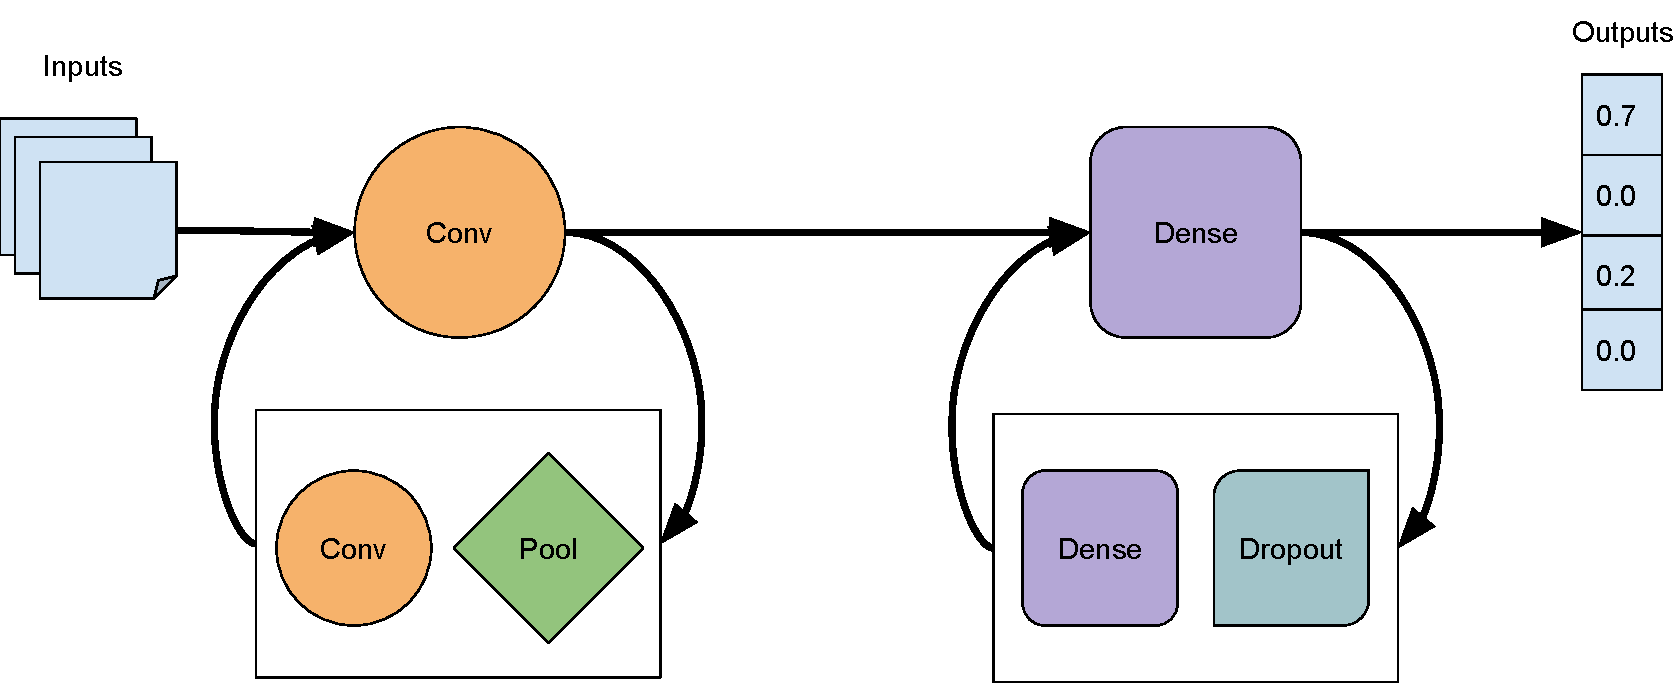
\includegraphics[width=\linewidth]{images/mapping-example.pdf}
	\caption{Example of mapping expansion of a CNN model.}
	\label{fig:cnn-map-scheme}
\end{figure}


%The way Keras can be used to build CNN models is very simple. We can create a \textit{Sequential} model, that is a linear stack of layers, and add the desired components. 

%Figure \ref{fig:cnn-model} shows an example of a simple CNN. It is also possible to save a model to a \textit{json} format, as well as load a model, but not the weights, from a \textit{json} file.

In the Grammatical Evolution, a solution is a list of integer values, and the mapping function will translate the solution into a CNN model using the components and parameters defined in the BNF grammar. The translation occurs by replacing non-terminal rules, following the left-most replacement rule, until all non-terminal are replaced by terminal rules. The way that productions are selected to replace a given non-terminal is by applying the mathematical \textit{mod} operator as:

\begin{equation}\label{eq:replace-eq}
	GR = sv~MOD~np
\end{equation}


where $GR$ is the chosen grammar rule resulted from the $MOD$ operation between solution value ($sv$) and the number of possible productions for that rule ($np$). Table \ref{tab:exp-example} shows an example of the mapping process of the solution [0, 13, 4, 20, 3, 5, 5, 9, 2] into a CNN. The `\&' symbol represents ``empty''.


\begin{table}[!htb]
	\small
	\caption{Grammar expansion example}
	\begin{tabular}{c|c|c|c|l}
		\hline
		step & value &   input   &   mod    & output                                                \\ \hline
		 1   &   0   &   <cnn>   & 0 mod 1  & <conv><c\_lay><d\_lay><dense>                         \\
		 2   &  13   &  <conv>   & 13 mod 1 & `Conv'<filters><k\_size><actv><c\_lay><d\_lay><dense> \\
		 3   &   4   & <filters> & 4 mod 2  & `Conv'`32'<k\_size><actv><c\_lay><d\_lay><dense>      \\
		 4   &  20   & <k\_size> & 20 mod 2 & `Conv'`32'`(3, 3)'<actv><c\_lay><d\_lay><dense>       \\
		 5   &   3   &  <actv>   & 3 mod 3  & `Conv'`32'`(3, 3)'`relu'<c\_lay><d\_lay><dense>       \\
		 6   &   5   & <c\_lay>  & 5 mod 3  & `Conv'`32'`(3, 3)'`relu'`\&'<d\_lay><dense>           \\
		 7   &   5   & <d\_lay>  & 5 mod 3  & `Conv'`32'`(3, 3)'`relu'`\&'`\&'<dense>               \\
		 8   &   9   &  <dense>  & 9 mod 1  & `Conv'`32'`(3, 3)'`relu'`\&'`\&'`Dense'<units>        \\
		 9   &   2   &  <units>  & 2 mod 2  & `Conv'`32'`(3, 3)'`relu'`\&'`\&'`Dense'`32'           \\ \hline
	\end{tabular}
	\label{tab:exp-example}
\end{table}


After the mapping, we get a list of strings that defines which components the CNN will have. From this list we can built a \textit{json} structure that will later be used to built the model in Keras. The \textit{json} structure will look like the example in Figure \ref{fig:json-example}. As mentioned before, some rules are applied to ensure that valid models will be built more often. In this example, the \textit{Convolution} node gained an extra parameter called ``input shape'' related to the problem, that were images 28x28 grayscale, then a \textit{Flatten} layer is added just before the first \textit{Dense} layer, as well as the number of units in the last layer was changed to the number of classes of the problem (10), and also an activation function was added with the \textit{Softmax} function.


\begin{figure}[!htb]
	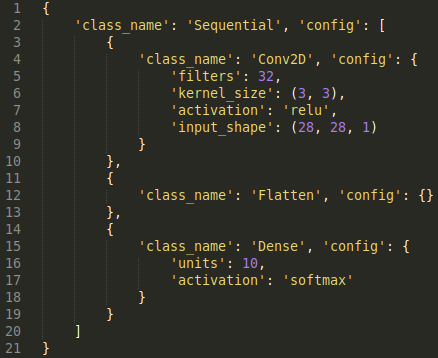
\includegraphics[width=\linewidth]{images/json-example.png}
	\caption{Example of JSON structure that represents the result of the mapping.}
	\label{fig:json-example}
\end{figure}


Finally, the CNN model is built by passing the \textit{json} to a Keras function called \textit{model\_from\_json} which output is a \textit{model} Sequential object with the components defined by the mapping performed before. The correspondent model can be seen in Figure \ref{fig:model-example} if it was built using the Keras syntax.


\begin{figure}[!htb]
	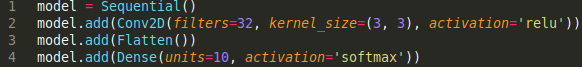
\includegraphics[width=\linewidth]{images/model-example.png}
	\caption{Example of CNN model built using Keras.}
	\label{fig:model-example}
\end{figure}


\subsection{Search}


The search engine is responsible to create, modify and evaluate solutions in order to increase the chances of finding a good solution that performs well on a given problem. The most common search algorithm used in GE is the Genetic Algorithm (GA). The GA is an algorithm designed based on the studies on the evolution of species, having genetic operators like selection, crossover and mutation as tools to combine and modify solutions.


\bibliographystyle{plain}
\bibliography{referencias}

\end{document}